%---
\section{Inner Detector and Cryogenics System}
\label{sec:TPCCryo}


%---
\subsection{\DSks\ \LArTPC}  
\label{sec:TPC}


The \DSk\ \LArTPC\ is the dark matter detector and the central element of the experiment, with all auxiliary detectors and systems specified and designed in support of it.  The \DSks\ \LArTPC\ will use \DSkCryogenicsCapableLArMass\ of \LAr\ extracted from an underground source as the target material for \WIMP\ detection.   An ultra-pure acrylic vessel is used to contain the \LAr.  Features directly fabricated onto the inner surfaces of the acrylic vessel will form the \TPC\ itself.  These feature are the \TPC\ field cage system, the anode and the cathode and are implemented on the acrylic panels with a commercial conductive polymer coating, called \Clevios.  Use of this coating eliminates the use of metal conductive materials. 

The same pure acrylic material, in the form of \DSkPMMATPCBackPanelThicknessESR\ thick sheets, is used to hold the Enhanced Specular Reflector (\ESR) reflector foils installed to maximize light collection. The \TPC\ is designed such that all the inner surfaces facing the active volume are coated with \TPB, a wavelength shifter, to ensure the complete conversion of the \ArWaveLength\ argon scintillation light to \TPBWaveLength, where the \SiPMs' peak in their PDE.  Two identical photosensor arrays of \DSkTilesHalfNumber\ channels each are placed on top and bottom of the \TPC, but outside of the acrylic vessel. The \TPC\ is mounted inside a neutron veto detector, whose most important component is a \DSkPMMAVetoPanelThickness\ thick, gadolinium loaded, acrylic shell that completely incapsulates the \TPC. This plastic shell defines two \DSkVetoLArThickness\ thick active volumes, respectively named the inner and outer buffer, filled with liquid \AAr. The buffers are further segmented with \ESR, also coated with \TPB. The whole apparatus is placed inside a light and electromagnetic shield barrier, contained in the \pDUNE-like cryostat filled with \AAr.

\begin{table}
\rowcolors{3}{gray!35}{}
\centering
\begin{tabular}{lc}
\hline
\hline
{\bf \DSks\ \TPC\  Dimensions} 		&\\
\hline
\TPC\ Drift Length					&\DSkActiveHeight\\
Octagonal Inscribed Circle Diameter	&\DSkActiveDiameter\\ 
Total \LAr\ Mass 					&\DSkTotalMass\\
Active \LAr\ Mass 					&\DSkActiveMass\\
Fiducial Cut Distance (vertical)	&\DSkVetoFVTPCcutz\\
Fiducial Cut Distance (radial)		&\DSkVetoFVTPCcut\\
Fiducial \LAr\ Mass 				&\DSkFiducialMass\\
\hline
{\bf Nominal \TPC\ Fields and Settings}
									&\cellcolor{white}\\
\hline
Drift Field 						&\DSkDriftField\\
Extraction Field  					&\DSkExtractionField\\
Luminescence Field 					&\DSkElectroLuminescenceField\\
Cathode Voltage 					&\DSkCathodePotential\\
Extraction Grid Voltage		  		&\DSkGridPotential\\
Anode Voltage  						&\DSkAnodePotential\\
Gas Pocket Thickness  				&\DSkGasPocketThickness\\
Grid Wire Spacing  					&\DSkLArOverGridPitch\\
Grid Optical Transparency  			&\DSkGridTrasparency\\
\hline
{\bf \SiPM\ \DSkPdm}				&\cellcolor{white}\\
\hline
Number of \DSkPdm\ on \TPC\ Top		&\DSkTilesHalfNumber\\
Number of \DSkPdm\ on \TPC\ Bottom	&\DSkTilesHalfNumber\\
\DSkPdm\ Effective Area 			&\DSkTileAreaStd\\ 
\hline
\end{tabular}
\caption[\DSks\ \LArTPC\ detector parameters]{\DSks\ \LArTPC\ detector parameters.}
\label{tab:LArTPC-Parameters}
\end{table}

{\bf Sealed \PMMA\ Vessel:} An acrylic (\PMMA) vessel will be used to confine the \UAr\ rather than a metallic vessel, since \PMMA\ is extremely radiopure, resulting in a residual neutron background estimated to be \DSkVetoPMMANeutronResidualBackground\ for the exposure of \DSkExtendedExposure.  As described above, the \TPC\ active volume is confined in all directions by the sealed \PMMA\ vessel that is formed by bonded plates or panels. In order to use the \UAr\ more efficiently, all the \UAr\ will be sealed in this \PMMA\ vessel, so that no other external vessel will be required (as shown in Figure~\ref{fig:TPC_acrylic}).  The body of the \PMMA\ vessel will be fused together by \DSkPMMATPCThickness\ thick acrylic plates, and then flanged and sealed with the top and the bottom lid, that serve as the anode plate and cathode plate of the \TPC, respectively.

\begin{figure}[!thbp]
\centering
\includegraphics[width=\columnwidth]{./Figures/TPC-acrylic-vessel-design.pdf}
\caption[Artist rendering of the \PMMA\ vessel and the \TPC]{Artist rendering of the \PMMA\ vessel and the \TPC.}
\label{fig:TPC_acrylic}
\end{figure}

The ESR-acrylic reflector panels are located inside the acrylic vessel. The top and bottom \DSkPdm\ arrays are placed outside of the acrylic vessel, immersed in the \AAr\ of the neutron veto detector. \DSkPdm\ arrays will be isolated from any light generated in the veto detector.  In this way, \DSkActiveMassRatio\ of the total argon is active, resulting in the most efficient usage of \UAr. All cables, \HVFTs, and most mechanical structures are moved outside of the \UAr\ volume as well, resulting in less outgassing and hence higher purity of the \UAr. 

The \HV\ Cathode connection through the acrylic vessel is being studied and a new design will be tested to adapt the cable connection to the cathode itself. The acrylic vessel design integrates the \HV\ connection so that the contact point is outside the vessel. In this case, both the \HV\ cable and the \HVFT\ are in the \AAr\ volume. The \HVFT\ will penetrate through the veto cryostat.

A commercial conductive and transparent Polymer coating, \Clevios, is found to be a very promising alternative to the traditionally used indium tin oxide (\ITO) thin film coating. \Clevios\ is being used in industrial applications such as transparent electrodes for touch panels and printed electronics. The main advantage of \Clevios\ is its composition.  Being a water-based solution, the large-area coating needed for the anode and cathode will be easier to accomplish with respect to an \ITO\ coating.  A sample of \CleviosFirstTestSampleMass\ has been procured for the radioactivity assay. The initial ICP-MS assay results from PNNL are encouraging, and further analysis of Rn emanation is scheduled at Krakow. In terms of the optics, three coating samples of \Clevios\ on acrylic plates were provided by The Heraeus Company. The wet coating thickness of each sample is \CleviosSampleThicknessFour, \CleviosSampleThicknessEight\ and \CleviosSampleThicknessTwelve, respectively, and their transparency has been measured at Princeton University. A \CleviosTestAbsorptionFour\ absorption at \DSfPMTWaveLength\ was observed for a \CleviosSampleThicknessFour\ thick \Clevios\ layer, which is a good result comparable to the \DSkITOTransparency\ transparency of \ITO\ measured in \DSfs. Further studies, including coated thickness resistivity, \TPB\ coating on \Clevios, and durability in \LAr\ are ongoing. Besides the anode and cathode, the new design replaces the bulky copper field shaping rings with \Clevios\ conductive coatings. Consequently, the use of this polymer will reduce the expected background, as well as the total cost, and make the fabrication and installation of the \TPC\ simpler. 

{\bf LArTPC Size Consideration:} Since the \SiPM\ tiles are all square shaped, the \DSks\ \TPC\ will be an octagonal shape to best fit the coverage of the \DSkPdm, while optimizing the fiducial mass.  The size of the \TPC\ is determined by the patterning strategy of the \SiPMs, driven by the design size of the square and triangular motherboards (SQB and TRB, respectively).  Figure~\ref{fig:TPC-SiPM_pattern} shows the current \SiPM\ pattern strategy for both the top and bottom arrays. Each array consists of \DSkArraySQBNumber\ \SQBs\ and \DSkArrayTRBNumber\ \TRBs. Each \TRB\ contains \DSkTRBPdmsNumber\ \DSkPdms\ and each \SQB\ contains \DSkSQBPdmsNumber\ \DSkPdms, as shown in Figure~\ref{fig:3D-TRB-SQB}. Thus, the number of \DSkPdms\ used in each array is \DSkTilesHalfNumber, while the total number envisioned in the \TPC\ is \DSkTilesNumber.  Based upon this pattern strategy, and considering that the edge of the active volume of the \TPC\ will shrink about \DSkEdgeActiveVolumeShrinkage\ from the edge of the \SiPM\ array, the distance from edge to edge of the octagonal active volume will be \DSkActiveDiameter.  The height of the \TPC\ will be \DSkTPCHeight. With this design, the total mass of \LAr\ in the active volume and fiducial volume (with \DSkVetoFVTPCcutz\ vertical and \DSkVetoFVTPCcut\ lateral cuts) are \DSkActiveMass\ and \DSkFiducialMass\ respectively. 

\begin{figure}[t!]
\centering
\includegraphics[width=\columnwidth]{Figures/TPC-SiPM_pattern.png}
\caption[\DSkPdm\ patterning scheme]{Patterning scheme for the \DSkPdms.  Pink lines indicate the edges of the \TPC\ active volume.}
\label{fig:TPC-SiPM_pattern}
\end{figure} 

{\bf Reflector Panel:} In order to get rid of the conventional \PTFE\ reflectors, which would be the predominant source of neutron background and Cherenkov background due to the enormous mass required for \DSks, ESR foils will be used as the \TPC\ reflector. The ESR is a thin layer foil which has reflectivity of \DSkESRReflectivity\ for \DSfPMTWaveLength\ light, with a thickness of only \DSkESRThickness.  In order to hold the ESR foils in place and maintain their flatness during the operations, \DSkPMMATPCBackPanelThicknessESR\ thick UVT acrylic sheets will be used. The thickness of the backside acrylic sheet is chosen to be \DSkPMMATPCBackPanelThicknessESR, providing the panels with enough strength to maintain the flatness of the ESR foils. %All the Cherenkov light introduced by this acrylic sheet and any other material outside will be blocked by the ESR foil. 
The surface of each ESR foil facing the active \LAr\ volume will be coated with \TPB. 

\begin{figure}[t!]
\includegraphics[width=0.49\textwidth]{./Figures/MB_TRB.png}
\includegraphics[width=0.49\textwidth]{./Figures/MB_SQB.png}
\caption[\DSks\ \DSkPdm\ motherboard designs]{Schematic drawings of the two types of \DSks\ \DSkPdm\ motherboard arrangements.  {\bf Left:} triangular with \DSkTRBPdmsNumber\ \DSkPdms\ arranged for center and edge placement.  {\bf Right:} square with \DSkSQBPdmsNumber\ \DSkPdms.}
\label{fig:3D-TRB-SQB}
\end{figure}

The entire reflector panel of the \TPC\ is shown in Figure~\ref{fig:re_panel}. The ESR mountings are strategically arranged such that no gaps can develop during the cool down of the \TPC, hence guaranteeing \DSkTPBCoverage\ \TPB\ coverage. Each ESR-acrylic sub assembly will be fixed by several acrylic screws, with the screw heads facing the active volume. To avoid losing any light, each head of the screw will also be coated with \TPB. By design, some space is left between the acrylic and the ESR to allow venting of any gas during the filling with \LAr, but also to allow the \LAr\ to fill the space between the back of the ESR and the acrylic panel. The flat and corner assemblies will be mounted on the field cage, which is attached to another set of acrylic structures by \PTFE\ screws. The ESR holding panels are not connected at the corners in order to accommodate the shrinkage when the assemblies are cooled to \LAr\ temperature. Overlaps between ESR foils at each joint are also designed for the same reason. A small mock-up to mimic the shrinkage has been built at UC Davis, whose results have confirmed the design concept. Repeated tests in liquid nitrogen showed that all parts moved in the desired way during cooling down and warming up, which proves the design idea.

\begin{figure}[t!]
\centering
\includegraphics[width=\columnwidth]{./Figures/TPC-reflector_panel.png}
\caption[3D model of the full \DSks\ \LArTPC\ reflector panels system]{3D model of the full \DSks\ \LArTPC\ reflector panels system.}
\label{fig:re_panel}
\end{figure}

{\bf Field Region:} Within the sealed acrylic vessel, the electrode features of the \TPC\ are realized using the \Clevios\ conductive polymer coated directly onto the acrylic vessel. The inner surface of the acrylic vessel will be machined with grooves such that recessed areas have geometries similar to an electrode ring, and when coated with the \Clevios\ comprise the \TPC\ field-shaping rings that are highly uniform across the height of the \TPC.  

The relative permittivity of \LAr\ and \GAr\ are \LArRelativePermittivity\ and \GArRelativePermittivity, respectively.  By applying electric potentials of zero, \DSkGridPotential, and \DSkCathodePotential\ to the anode, extraction grid and cathode, respectively, three different field regions are formed in the \TPC:

\begin{compactitem}
\item The uniform drift field of \DSkDriftField\ in the liquid phase, formed by the geometry of the field cage. The drift distance between the cathode \Clevios\ layer and the extraction grid is \DSkTPCHeight;
\item The extraction field in the liquid phase above the grid is \DSkExtractionField. The distance between the extraction grid and the surface of the \LAr\ is \DSkLArOverGridThickness;
\item The electroluminescence field in the gas phase is \DSkElectroLuminescenceField. The gas gap between the surface of the \LAr\ and the \Clevios\ layer acting as the anode is \DSkGasPocketThickness\ thick.
\end{compactitem}

These values are based on the settings used for \DSfs, while since the \DSks\ gas pocket will be operating at a higher pressure, the extraction and luminescence fields will be scaled by the ratio of the electric field to the pressure of the gas pocket. The final values to be used will be confirmed with the \DSps\ detector that is designed to confirm final design choices for the \DSks\ \LArTPC.

As the top boundary of the active volume, a \DSkPMMATPCThickness\ thick acrylic window serves as the diving bell to maintain a stable gas pocket. A thin layer of \Clevios\ conductive polymer is coated on the inner surface to act as the anode and a layer of \TPB\ coated onto the \Clevios\ layer to shift the scintillation light wavelength. The \Clevios\ layer coating geometry is optimized for gas pocket electroluminescence field uniformity, as shown in the left panel of Figure~\ref{fig:TPC_anode_cathode}. Right below the liquid surface is the extraction grid, composed of stainless steel wires (not shown in figure) stretched in parallel with \DSkWirePitch\ spacing and held in place via small posts set into a stainless steel frame. Slots going in the radial direction and on the rim of the acrylic diving bell act as a concentric guide, to compensate the different thermal expansion coefficients between the acrylic and stainless steel while maintaining precise alignment.  The \LAr\ level will be maintained at the top surface of the grid frame.  Suitable tensions will be pre-loaded on each of the grid wires to minimize the sagging, an effect that would distort the electroluminescence field. The frame must be stiff enough to sustain the total tension load of all wires, while having as little mass as possible. Both simulation studies and prototyping tests are well underway and have presented a feasible design for the extraction grid.

\begin{figure}[t!]
\centering
\includegraphics[width=0.49\columnwidth]{./Figures/TPC-anode.pdf}
\includegraphics[width=0.49\columnwidth]{./Figures/TPC-cathode.pdf}
\caption[\DSks\ \LArTPC\ anode and cathode regions]{{\bf Left:} 3D model of the \LArTPC\ anode and extraction grid region.  {\bf Right:} 3D model of the \LArTPC\ cathode region.}
\label{fig:TPC_anode_cathode}
\end{figure}

The bottom boundary of the active volume, shown in the right panel Figure~\ref{fig:TPC_anode_cathode}, is a \DSkPMMATPCThickness\ thick acrylic window coated with a thin layer of \Clevios\ on both sides. A layer of \TPB\ will be coated on the top \Clevios\ layer for wavelength shifting. The edge of the top \Clevios\ layer is in contact with a C-profile feature on the walls of the acrylic vessel, which acts as a field shaping ring and smooths the electric field lines in the corner of the cathode region. Similarly, the bottom \Clevios\ layer is in contact with a smoothing-profile solid guard copper ring to provide connection for the ground bias and electric field minimization. The  \DSkPMMATPCThickness\ thick acrylic window can easily sustain the applied electric field with this design. Figure~\ref{fig:TPC_Field} shows the full field mapping modeled with the COMSOL Multiphysics software. Since the vessel is sealed, there is no path for HV to break through the acrylic at the cathode region. To confirm this, a full scale mock-up will be built to confirm the cathode HV delivery method around the acrylic vessel bottom.   The bottom surface of the cathode acrylic window will have a convex shape to avoid bubble accumulation.  Any bubbles generated by the bottom photon detector array, or any other parts, will be driven outwards and rise to the top of the \AAr\ cryostat.


\begin{figure}[!t]
\centering
\includegraphics[height=0.95\textheight]{./Figures/TPC-Field-Map.PNG}
\caption[Simulated electric field mapping of the \DSks\ \LArTPC]{Equipotential lines mapping in the \DSks\ \TPC\ showing an extremely uniform field distribution, modeled with the COMSOL Multiphysics program.  Parameter settings for the calculation are those defined in \reftab{LArTPC-Parameters}.}
\label{fig:TPC_Field}
\end{figure}

A one tonne-scale prototype with full features of the \DSk\ \TPC\ will then be built to validate the design comprehensively. General considerations, such as the requirements of surface and bulk contamination, coating procedures, handling and bonding of acrylic, are based on knowledge available within the \GADMC. Detailed plans and procedures are currently being developed. All mock-up designs and tests will use final \DSks\ geometries and full size components in order to confirm the validity of the final \DSks\ mechanical design and functional parameters. The \DSks\ \LArTPC\ parameters are summarized in Table~\ref{tab:LArTPC-Parameters}.


%---
\subsection{Cryogenics} 
\label{sec:Cryogenics}

\begin{table*}[!t]
\rowcolors{3}{gray!35}{}
\centering
\begin{tabular}{lc}
\hline\hline
{\bf Parameter}															&{\bf Value}\\ 
\hline\hline
{\bf \pDUNE\ Cryostat parameters for \AAr} 								&\\
\hline\hline
\pDUNE\ Cryostat inner width											&\pDUNECryostatInnerWidth\\
\pDUNE\ Cryostat inner height											&\pDUNECryostatInnerHeight\\
\LAr\ height in \pDUNE\ Cryostat										&\pDUNELiquidHeight\\
Total \AAr\ in \pDUNE\ Cryostat 										&\pDUNELArMass\\
\pDUNE\ Cryostat insulation per unit area								&\pDUNEWallHeatLeakArea\\
Thermal Heat Load of \pDUNE\ Cryostat 									&\pDUNECryostatHeatLoad\\
\TPC\ \DSkPdm\ Cold Electronics Power									&\TPCPdmPower\\
Veto \DSkPdm\ Cold Electronics Power 									&\VetoPdmPower\\
\AAr\ System Design Mass Circulation Speed 								&\DSkCryogenicsAArFlowTotal\\
{Minimum heat recovery efficiency of \AAr\ heat exchanger}				&$>$\DSkCryogenicsRecoveryExchangerEfficiency\\
\AAr\ Turn Over Time 													&\DSkAArTurnOverTime\\
{Total Cooling Power Required}											&\DSkAArCryogenicsTotalPower\\
\LAr\ boiling threshold at \DSkLArBoilingThresholdDepth\ depth			&\DSkLArBoilingThreshold\\
Minimum \AAr\ condenser cooling power to hold \LAr\ inventory			&\pDUNECryostatHeatLoad\\
\pDUNE\ \AAr\ top pressure												&\pDUNEAArTopPressure\\
\hline\hline
{\bf \TPC\ Cryogenics Parameters for \UAr} 								&\\
\hline\hline
Total \UAr\ mass during normal operation								&\DSkTotalMass\\
\TPC\ \UAr\ Cryogenics Design Mass Circulation Speed 					& \DSkCryogenicsGasFlowTotal\\
{Minimum heat recovery efficiency of \UAr\ heat exchanger}				&$>$\DSkCryogenicsRecoveryExchangerEfficiency\\
\UAr\ Turn Over Time 													&\DSkUArTurnOverTime\\
{Total Cooling Power Required for \UAr}									&\DSkUArCryogenicsTotalPower\\
\UAr\ Turn Over Time 													&\DSkUArTurnOverTime\\
																		&$>$\DSkCryogenicsDSfElectronMeanLife\\
\multirow{-2}{*}{\UAr\ electron lifetime required for stable \STwo\ generation}	\cellcolor{gray!35}
																		&\cellcolor{gray!35}($<$\DSfUArChemicalPurity\ \ce{O2} equiv.)\\	
\cellcolor{white}Pressure stability achieved in \DSf\					&\cellcolor{white}\DSfCryogenicsPressureStability\ (RMS)\\
Nominal flow rate of single \DSk\ \GAr\ circulation pump				&\DSkCryogenicsQdriveSpeed\\
Total mass of \LIN\ storage in cooling system							&\DSkCryogenicsLINStorageMass\\
Efficiency of radon purification by activated charcoal trap				&\SI{<2}{\micro\becquerel\per\kilo\gram} after trap\\
{ Maximum required helium leak rate at all welds and joints}			&\DSkCryogenicsHeliumLeakCheckRequirement\\
\hline
\end{tabular}
\caption[\DSk\ cryogenics system parameters]{\DSk\ cryogenics system parameters.}
\label{tab:Cryo-parameters}
\end{table*}

The main system parameters of the cryogenics system are given in Table~\ref{tab:Cryo-parameters}.  The parameters that are listed in bold are considered to be system requirements, most often driven from experience gained during operations of the \DSfs\ cryogenics system.

The cryogenics system is derived from the successful scheme of the \DSfs\ cryogenics and gas handling system. Additional lab tests, already performed over the past 4 years, demonstrated individual or integrated features required for the performance of the control system and the safety of the large amount of \UAr\ in the \DSk\ system. A full P\&ID diagram is already developed as shown in Figure~\ref{fig:DSCryo}. There are two major linked systems: one for the \AAr\ in the veto shield inside the \pDUNE\ cryostat and one for the \UAr\ in the sealed acrylic vessel for the \LArTPC.  The \AAr\ cryogenics system can be the same as the demonstrated  \pDUNE\  system already built at \CERN, or an optimized version specific for the \LNGS\ installation. The \UAr\ cryogenics system for the \TPC\ will be an upgraded system based on \DSfs. The \pDUNE\ cryostat is a passively insulated system so that its thermal load is not subject to the availability of the electric power. Liquid nitrogen is the primary cooling source of the entire cryogenics system. A minimum storage of the liquid nitrogen is maintained such that the system will be protected during power failure mode. A full scale version of the condenser box for the underground argon has already been designed and all parts procured. The cryogenics test of the condenser is planned at the \CERN\ cryogenic division in summer 2019.

Heat exchangers are strategically placed throughout the system for \LAr\ filling and \LAr\ removal at the various required speeds for the different operational modes. The continuous argon circulation for purification is driven by a set of specialized gas argon pumps (developed within the collaboration). Combined with the integrated heat exchanger systems, the system can handle high circulation rates (\DSkCryogenicsAArFlowTotal\ \AAr, and \DSkCryogenicsGasFlowTotal\ \UAr) drawing either, or both, liquid and gas phase argon to effectively remove electronegative impurities.  The designed P\&ID system allows the use of SAES hot getter to effectively remove \ce{N_2}, \ce{CO_2}, and \ce{O_2}. The total cooling power of the cryogenics system is designed to handle the total heat load from the power dissipated by the cold electronics operating inside the liquid argon volume.

The cryogenics system for the \LArTPC\ in \DSks\ shares the same principle as that fully demonstrated in \DSfs, which has been running smoothly for five years. The long-term \TPC\ pressure stability, an essential parameter for \STwo\ resolution, has been achieved with incredible success, quantified as \DSfCryogenicsPressureStability\ RMS.  A drift electron lifetime of \DSfElectronMeanLife\ has been achieved, resulting in an oxygen contamination in \LAr\ of less than \DSfUArChemicalPurity, which is greatly beneficial to the low-mass dark matter search, as recently published in~\cite{Agnes:2018fg, Agnes:2018ft}. The immunity to total power failure (including UPS system failure), as tested in the commissioning phase and verified by a recent accident of total \LNGS\ blackout, secures the safety of the entire \LArTPC, especially the valuable \UAr. 

\begin{figure}[!t]
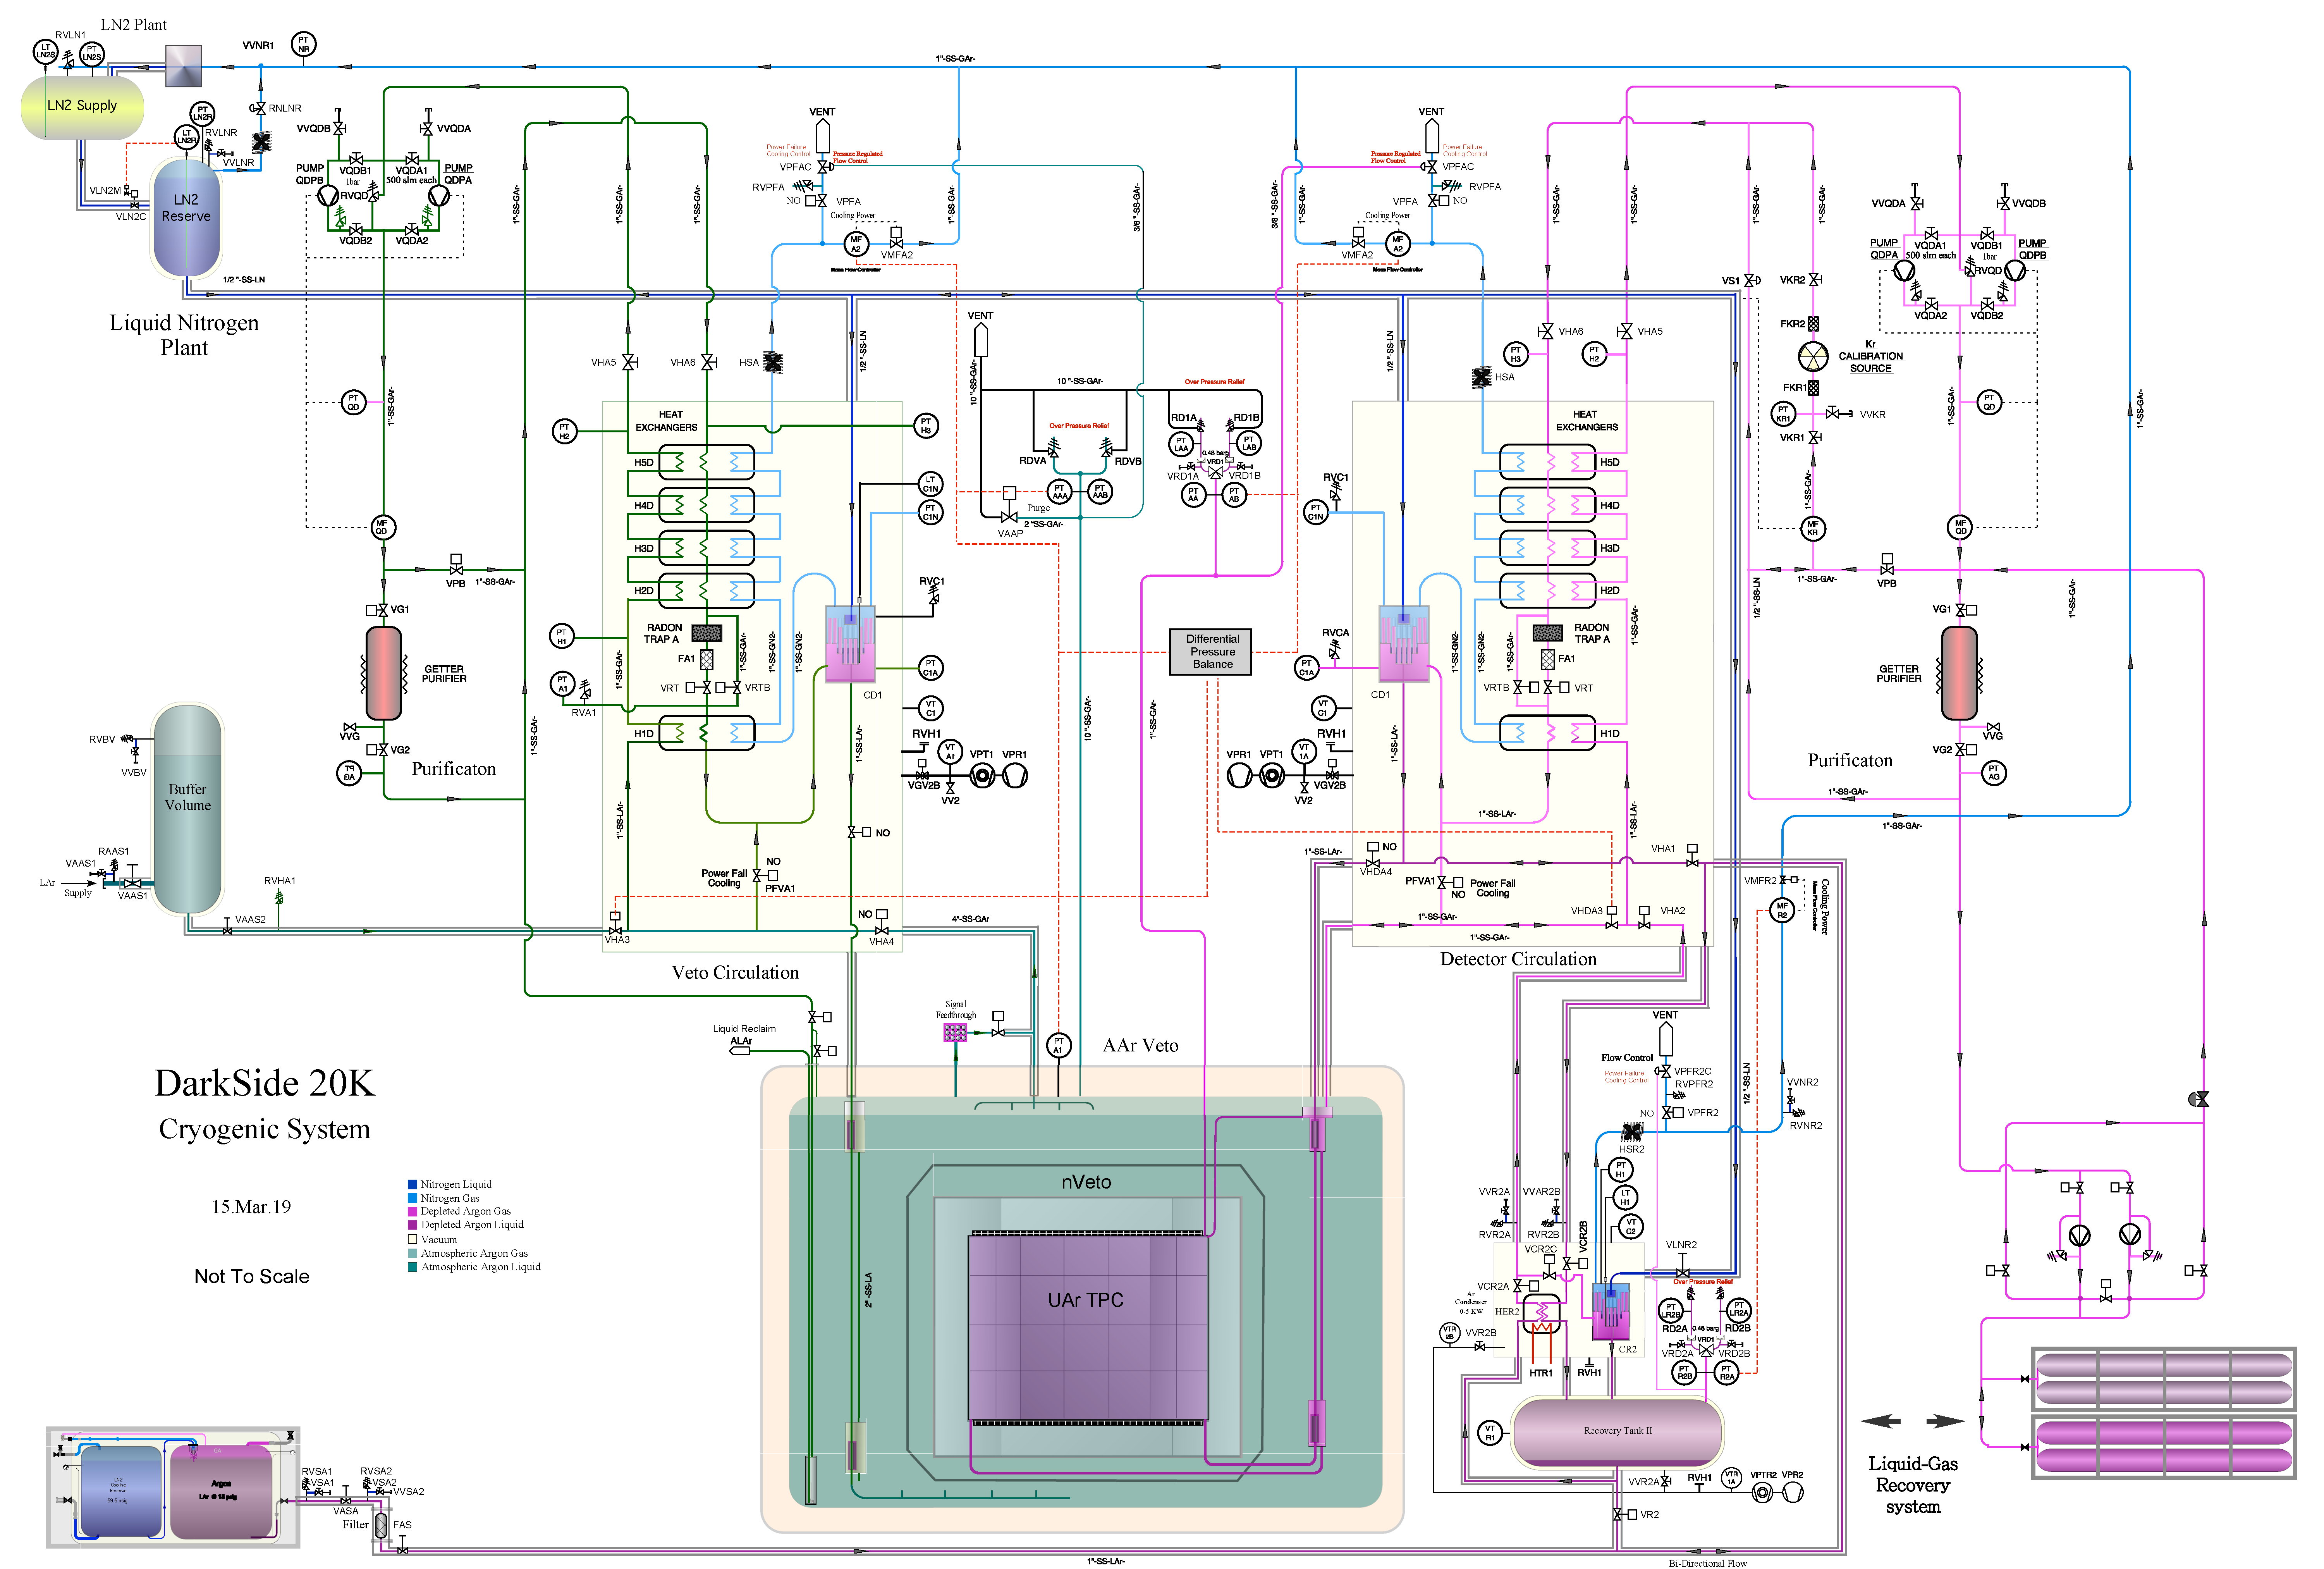
\includegraphics[rotate=90,height=0.95\textheight]{./Figures/DarkSide-20k-Cry-P&ID.pdf}
\caption[\DSks\ cryogenics system P\&ID]{\DSks\ cryogenics system P\&ID.}
\label{fig:DSCryo}
\end{figure}

\begin{figure}[!t]
\includegraphics[height=0.95\textheight]{./Figures/DSk-UArCryogenics.PDF}
\caption[\DSks\ condenser box]{\DSks\ condenser box.}
\label{fig:DSCondenser}
\end{figure}

The features of the \DSfs\ cryogenics system are fully implemented into the \DSks\ system, not only by simply scaling up the argon volume, but also upgrades based on experience and lessons learned.  A major improvement is to increase the circulation speed to the required \DSkCryogenicsGasFlowTotal, to initially reach the purity requirement of \LAr\ in a couple of turn-over times of \DSkUArTurnOverTime.  Another major improvement is to increase the cooling power needed to accommodate such a large circulation speed.  A full-size prototype \LAr\ condenser, the core component in the cryogenics system, has been built and tested at UCLA, and a cooling power of \DSkCryogenicsCondenserCoolingPowerMaxTested\ (latent heat only) has been achieved, nearly twice that needed for the \DSks\ \UAr\ cooling requirement.  The main components of the \UAr\ cryogenics system condenser box have already arrived at CERN and are ready for welding and the first test to follow in summer 2019.   

The \UAr\ cryogenics system is made up of several sub-systems (while the \AAr\ system will be similar except at larger scale in volume and power, but with lower requirements on purity): the liquid argon handling system, the liquid nitrogen reserve system, the purification system, the cold box, the gas circulation pump, the recovery and storage system, the integrated heat exchanger system, and heat exchangers close to the \TPC.  The overall schematic is shown in Figure~\ref{fig:DSCryo}, including the \AAr\ cryogenics system for the veto detector, which employs the same principle.  Two cryogenics systems share the same liquid nitrogen reserve loop, but have separate argon loops of \UAr\ and \AAr, respectively.  Also shown in the figure is the condenser box integrated with the heat exchangers and inline radon trap. 

The \LAr\ handling system delivers the clean radon-free \UAr, which is initially stored in the recovery storage system capable of storing the full target of \UAr\ for \DSks.  Two options are being considered, full liquid phase storage or gas phase high-pressure storage. The gas handling system will be adopted to either solution in order to pre-purify the \UAr\ before filling the TPC volume.   The system is also designed such that the \UAr\ can be recuperated from the inner detector to the recovery system, as needed, if an emergency occurs or at the end of the experiment.

The \LIN\ reserve system is a closed loop with a \LIN\ plant located outside of Hall\,C and a few local liquid nitrogen dewars.  The system delivers liquid nitrogen as the source of cooling power to the condensers in the inner detector \UAr\ cryogenics system, the \AAr\ cryogenics system, and the recovery system, if liquid phase storage is chosen, and recuperates the boiled-off nitrogen gas to liquify it back into the \LIN\ system.  The \UAr\ purification system purifies the argon in gas phase during the circulation.  A commercial SAES getter system has already been proven to work well in \DSfs\ and an identified model with increased circulation capability will be used in \DSks.

The cold box, as shown in Figure~\ref{fig:DSCondenser}, is one of the key components of the \DSks\ cryogenics system, which contains all the major cryogenic handling components.  Apart from the condenser, the cold box contains five heat exchanger modules to efficiently pre-cool the argon gas by cold nitrogen gas and cold outgoing argon gas.  In this way the necessary cooling power is reduced dramatically.  The radon trap is placed between the coldest and the second coldest heat exchanger modules to ensure that the argon passing through is still in its gas phase, while at its lowest temperature, which maximizes the radon removal efficiency.  Eight cryogenic valves and several temperature and pressure sensors are also installed to control and monitor the system.  Tubings are chosen as \DSkCryogenicsTubesDiameter\ OD stainless steel, in order to accommodate the argon circulation speed up to \DSkCryogenicsGasFlowTotal. 

The stainless steel \LAr\ condenser contains \DSkCondenserTubeNumber\ \DSkCryogenicsCondenserTubesDiameter\ OD top-sealed tubes finely patterned on a thick plate as the thermal exchanging part of the condenser.  The condenser is therefore separated into the nitrogen volume on the top and the argon volume on the bottom.  A so-called {\it chicken feeder} is mounted at the end of the liquid nitrogen delivery tube to maintain a continuous liquid nitrogen dropping.  The flow of the evaporated nitrogen gas is monitored by a mass flow meter and adjusted by a control valve, both located at ambient temperature.  The control valve uses the \LArTPC\ pressure from both \UAr\ and \AAr\ as feedback signal to automatically adjust the evaporated nitrogen gas flow rate, which is essentially the cooling power of the condenser, hence in return maintains the \LArTPC\ pressure at the desired set point and balanced with \AAr\ system with an incredible stability, as demonstrated in \DSfs.

Based on the successful demonstration of the gas circulation pump in \DSfs, which provides a speed up to \DSfCryogenicsGasFlowLINBoost, the gas circulation pump of \DSks\ uses the similar design, relying on two components: linear motors and reed valves.  The linear motors, consisting of a piston and cylinder pair, can provide a continuously adjustable pumping power.  The reed valves guide the gas flow direction when the linear motors going back and forth.  Two balanced linear motors will be placed face to face, to counteract the vibration produced during the motor operation. The combination of the linear motors and the reed valve allows the pump to work in a frictionless condition, resulting in a long lifetime.  The initial fast circulation requires a speed of \DSkCryogenicsGasFlowTotal\ to achieve a good \UAr\ purity level, and then the circulation speed can be decreased to only maintain the purity and stability. This minimum flow could be very low since the \UAr\ system essentially is embedded in the \AAr\ system while all cold electronics are outside the \UAr\ volume so no cooling power is required. To achieve such a high circulation speed, flexibility of operations, as well as the ease of the pump development, two individual circulation pumps will be placed in parallel, each providing a circulation rate up to \DSkCryogenicsQdriveSpeed.  A full-size prototype circulation pump has been fabricated at UCLA and Princeton, and passed the initial tests.  It was shipped to \CERN\ and is being certified for the EU safety requirement. Once fully tested,  it will be integrated into the prototype cryogenics system for the full-system test.

The heat exchangers close to the TPC are basically large heat exchangers using many tubes as the thermal exchanging parts, similar to the concept of the \LAr\ condenser described above, but with a much increased thermal exchanging surface area.  Outgoing \LAr\ from the \LArTPC\ absorbs heat from the incoming liquid-gas mixture of purified argon here, boils off into gas phase, and then enters the circulation loop.  This heat exchanger is located above the \LArTPC\ and ensures that all outgoing argon above it will be in gas phase, avoiding otherwise a large argon head height coming directly from the \LArTPC\ to the lowest heat exchanger modules in the cold box.  This would result in an argon pressure below its triple point at some point in the argon loop and causing argon to freeze.  Another set of near TPC heat exchangers are strategically placed close to bottom level of the \UAr\ TPC for fast recovery during the draining stage. This lower level heat exchanger is completely passive during normal operations and only useful during the draining phase. The entire near TPC heat exchangers are immersed in \LAr\ inside the \pDUNE\ cryostat, which serves as a thermal bath for them.

The integration and tests of the full scale \UAr\ cryogenics system at \CERN\ is ongoing. The first pass FEA engineering has proven the design load is as anticipated and fabrication is officially approved. All condenser box components, large pneumatic cryogenics valves and associated auxiliary components are on site at CERN for integration. The full scale cryogenics test of the \DSk\ \UAr\ system will be performed over the summer of~2019.